\begin{flushright} {\tiny {\color{gray} pair\_q1p0stab.tex}} \end{flushright}
%~~~~~~~~~~~~~~~~~~~~~~~~~~~~~~~~~~~~~~~~~~~~~~~~~~~~~~~~~~~~~~~~~~~~~~~~~~~~~~~~~~~~~~~~~~~~~~~~~~

WARNING: this entire subsection is copied from an old document. It needs to be revised and 
updated. I intend to write a Stone implementing this element.

\Literature: Explore these 2 refs which I found after my q1p0-stab work of 2015 \cite{chke20,eguc03}

Many techniques have been proposed to stabilise this element:

\begin{itemize}
\item method ? : \cite{bbgs04},  \cite{bodg06} , \cite{bogl07}
\item stabilisation through macro-elements: \cite{fobo90}, \cite{leru86}, \cite{leta81}
\item local jump stabilisation: \cite{sike90}, \cite{kesi92,vibo92,qizh07,chri02,chco01,lisi12,lica06}
\item global jump stabilisation: \cite{hufr87}, \cite{nosi98}, \cite{dowa89} \cite{chco01}
\item supg like stabilisation: \cite{teos00}, \cite{tezd92,hufb86}
\item enrichment through velocity and/or pressure bubble function \cite{frol03}(only triangles)
\item additional (normal) velocity degrees of freedom on faces \cite{fofo85}, 
mentioned in \cite{sofo87}, \cite{fort81}.
adding 1 dof mid-side on each face with buble function \cite{rota87}
\end{itemize}

In effect, both jump stabilisation techniques provide an a-priori filter for the weakly unstable pressure modes associated 
with the Q1P0 element. The global jump stabilisation formulation introduces a pressure diffusion operator
that perturbs the incompressibility constraint. The global jump formulation insures mass conservation in a global  
sense since the null space of the stabilising matrix constains the constant-pressure vector. However, the global 
jump stabilisation smears the div-free constraint over a small region, i.e., the divergence is not 
zero at the element level \cite{chri00}.

The stability of mixed finite element methods boils down to properties of the null space of the matrix $\G$. 
An approximation is unstable if $\G \cdot \vec{\cal P} = \vec{0}$ where $\vec{\cal P}$ 
corresponds to some spurious pressure mode different from the constant value pressure.  
Note that if $\G\cdot \vec{\cal P} = \vec{0}$, then $(\vec{0},\vec{\cal P})^T$ is a null vector of 
the homogeneous system. 
The basic idea behind stabilization is to relax the incompressibility constraint in a special way so that 
this vector is no longer a null vector of the resulting coefficient matrix, and 
the discrete solutions satisfy rigorous error bounds. 
Stabilization is applicable to any mixed approximation method. 

Spatial discretisation of the Stokes equation using FD of FE results 
in large, sparse saddle-point systems of the form

\begin{equation}
\left(
\begin{array}{cc}
\K & \G \\
\G^T & -\C
\end{array}
\right)
\cdot
\left(
\begin{array}{c}
\vec{\cal V} \\ \vec{\cal P}
\end{array}
\right)
=
\left(
\begin{array}{c}
\vec{f} \\  \vec{h}
\end{array}
\right)
\end{equation}
where $\C$ is a stabilisation matrix to be stpecified.

The dimension of the $\C$ matrix is that of $h^{dim}/\eta$ where 
$h$ is the element size and $\eta$ a viscosity.







%----------------------------------------
\paragraph{Penalty approach}

The conventional way of computing a regularisation matrix $\C$
is to use a penalty formulation.
In the framework presented in \cite{sike90}, the standard penalty
method corresponds to the specific choice of
\[
C(q^h,p^h)=\epsilon \int_\Omega q^h p^h d\Omega = \epsilon {\bm M}_p
\]
with $\epsilon > 0$ and ${\bm M}_p$ is the pressure mass matrix. 
For a regular grid of squares with size $h$, it follows that 
\[
C_{ij}=0 \quad {\rm if} \; i\neq j
\quad\quad\quad
C_{ii}=\epsilon \int_{elt. i} d\Omega = h^2 \epsilon
\]
so that the stabilisation matrix is diagonal (see red matrix hereunder).

It is stressed here that the penalty technique does not stabilise an  
unstable mixed method \cite{sike90}. A small penalty parameter 
means that the original problem is solved quite accurately.

See \cite{cuss86} for some more details about the penalty method.

%-----------------------------------------------------
\paragraph{Global jump stabilisation}

Consider the stabilisation term
\[
C(q^h,p^h) = \beta h \sum_{s=1}^{N_s} \int_{\partial \Omega_s}[[ q^h ]]  [[p^h ]] ds
\]
in which $h$ is the mesh parameter (defined locally), $[[.]]$ is the jump operator,
and $\beta>0$ is a stabilising parameter. 
The summation is over all interior inter-element edges.

%from \cite{sike90}
To illustrate, consider element $9$ is the patch of equally  sized
squares represented here

\begin{center}
\begin{flushright} {\tiny {\color{gray} (tikz\_globaljump.tex)}} \end{flushright}
%~~~~~~~~~~~~~~~~~~~~~~~~~~~~~~~~~~~~~~~~~~~~~~~~~~~~~~~~~~~~~~~~~~~~~~~~~~~~~~~~~~~~~~~~~~~~~~~~~~

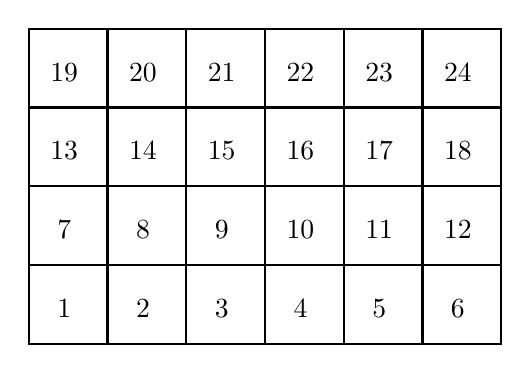
\begin{tikzpicture}
%\draw[step=0.5cm,gray,very thin] (0,0) grid (6,4); %background grid

\draw[thick] (0,0)--(6,0)--(6,4)--(0,4)--cycle;  

\draw[thick] (0,1)--(6,1);  
\draw[thick] (0,2)--(6,2);  
\draw[thick] (0,3)--(6,3);  

\draw[thick] (1,0)--(1,4);  
\draw[thick] (2,0)--(2,4);  
\draw[thick] (3,0)--(3,4);  
\draw[thick] (4,0)--(4,4);  
\draw[thick] (5,0)--(5,4);  

\node[] at (0.45,0.45) {1};
\node[] at (1.45,0.45) {2};
\node[] at (2.45,0.45) {3};
\node[] at (3.45,0.45) {4};
\node[] at (4.45,0.45) {5};
\node[] at (5.45,0.45) {6};

\node[] at (0.45,1.45) {7};
\node[] at (1.45,1.45) {8};
\node[] at (2.45,1.45) {9};
\node[] at (3.45,1.45) {10};
\node[] at (4.45,1.45) {11};
\node[] at (5.45,1.45) {12};

\node[] at (0.45,2.45) {13};
\node[] at (1.45,2.45) {14};
\node[] at (2.45,2.45) {15};
\node[] at (3.45,2.45) {16};
\node[] at (4.45,2.45) {17};
\node[] at (5.45,2.45) {18};

\node[] at (0.45,3.45) {19};
\node[] at (1.45,3.45) {20};
\node[] at (2.45,3.45) {21};
\node[] at (3.45,3.45) {22};
\node[] at (4.45,3.45) {23};
\node[] at (5.45,3.45) {24};

\end{tikzpicture}


\end{center}

The stabilisation term for this element involves the sum over its four neighbours:
\begin{eqnarray}
\beta h \sum_{s=1}^{4} \int_{\partial \Omega_s}[[ q^h ]]  [[p^h ]] ds
&=& \beta h^2 [ (p_9-p_3)+(p_9-p_8)+(p_9-p_{10})+(p_9-p_{15})   ]  \nn\\
&=& \beta h^2 ( 4 p_9-p_3 -p_8-p_{10} -p_{15})  \nn
\end{eqnarray}
The integral along each edge is simply the pressure difference across the edge 
multiplied by the edge surface/length which happens to be constant in this case.
This means that the in the matrix $\mathbb{C}$, there will be entries on the $9^{th}$
line at columns 3, 8, 10, and 15. 

Be careful, let us now turn to element 6: it has 2 neighbours (5 and 12), so that
the stabilisation term for this element involves the sum over its two neighbours:
\begin{eqnarray}
 \beta h^2 [ (p_6-p_5)+(p_6-p_{12})  ]  
&=& \beta h^2 ( 2 p_6-p_5 -p_{12} )  \nn
\end{eqnarray}

And looking now at element 23: it has three neighbours (17, 22, and 24), so that 
the stabilisation term for this element involves the sum over its three neighbours:
\begin{eqnarray}
\beta h^2 [ (p_{23}-p_{17})+(p_{23}-p_{22}) +(p_{23}-p_{24})  ] 
&=& \beta h^2 ( 3 p_{23}-p_{17} -p_{22} - p_{24} )  \nn
\end{eqnarray}


The resulting assembled $\C$ matrix is shown in green on the figure here after.

The global jump stabilisation is effective in
practice, although a careful choice of the parameter $\beta$
is required in order to prevent a loss of accuracy in the solution.
The only other deficiency is the fact that the global nature of the jump terms makes the method awkward to implement into existing codes
\footnote{I don't understand this remark}.\cite{sike90}

A general theoretical framework for analysing global stabilisation techniques is
presented in \cite{hufr87}.
Using this framework, optimum rates of convergence for the $Q_1\times P_0$
method stabilised with global jumps are established.

In \cite{cao03} the parameter $\beta$ is set to 1.

Note that this approach is somewhat linked to the idea of a pressure smoother 
via a discrete Laplace\footnote{\url{http://en.wikipedia.org/wiki/Discrete_Laplace_operator}}:
The Discrete Laplace operator is often used in image processing e.g. in edge detection and motion 
estimation applications. The discrete Laplacian is defined as the sum of the second derivatives Laplace 
and calculated as sum of differences over the nearest neighbours of the central pixel.
Here is an example of a 2D filter and it is of course similar in nature to the Global 
stabilisation stensil matrix:
\[
D^{(1)}=
\left[
\begin{array}{ccc}
0 &-1 &0\\
-1 &+4 &-1\\
0 &-1 &0
\end{array}
\right]
\]

Other filters can also be found:

\[
D^{(2)}=
\left[
\begin{array}{ccc}
-0.5 &-1 &-0.5\\
-1 &+6 &-1\\
-0.5 &-1 &-0.5
\end{array}
\right]
\quad\quad\quad
D^{(3)}=
\left[
\begin{array}{ccc}
-1 &-1 &-1\\
-1 &+8 &-1\\
-1 &-1 &-1
\end{array}
\right]
\quad\quad\quad
D^{(4)}=
\left[
\begin{array}{ccc}
1 & -2 & 1 \\
-2 & 4 & -2 \\
1 & -2 & 1 \\
\end{array}
\right]
\]


%-----------------------------------------------------------------------------------
\paragraph{Local jump stabilisation}

%sike90
The deficiencies of the global jump method can be overcome by  
a straightforward modification. Assume that the elements in  
can now be assembled into $N_m$ disjoint macro-elements 
of 2x2 elements, as shown in grey on the following figure: 

\begin{center}
\begin{flushright} {\tiny {\color{gray} (tikz\_localjump.tex)}} \end{flushright}
%~~~~~~~~~~~~~~~~~~~~~~~~~~~~~~~~~~~~~~~~~~~~~~~~~~~~~~~~~~~~~~~~~~~~~~~~~~~~~~~~~~~~~~~~~~~~~~~~~~


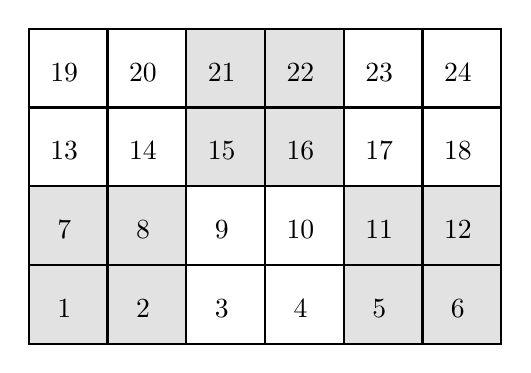
\begin{tikzpicture}
%\draw[step=0.5cm,gray,very thin] (0,0) grid (6,4); %background grid

\draw[fill=gray!23,gray!23](0,0) rectangle (2,2);
\draw[fill=gray!23,gray!23](2,2) rectangle (4,4);
\draw[fill=gray!23,gray!23](4,0) rectangle (6,2);

\draw[thick] (0,0)--(6,0)--(6,4)--(0,4)--cycle;  

\draw[thick] (0,1)--(6,1);  
\draw[thick] (0,2)--(6,2);  
\draw[thick] (0,3)--(6,3);  

\draw[thick] (1,0)--(1,4);  
\draw[thick] (2,0)--(2,4);  
\draw[thick] (3,0)--(3,4);  
\draw[thick] (4,0)--(4,4);  
\draw[thick] (5,0)--(5,4);  

\node[] at (0.45,0.45) {1};
\node[] at (1.45,0.45) {2};
\node[] at (2.45,0.45) {3};
\node[] at (3.45,0.45) {4};
\node[] at (4.45,0.45) {5};
\node[] at (5.45,0.45) {6};

\node[] at (0.45,1.45) {7};
\node[] at (1.45,1.45) {8};
\node[] at (2.45,1.45) {9};
\node[] at (3.45,1.45) {10};
\node[] at (4.45,1.45) {11};
\node[] at (5.45,1.45) {12};

\node[] at (0.45,2.45) {13};
\node[] at (1.45,2.45) {14};
\node[] at (2.45,2.45) {15};
\node[] at (3.45,2.45) {16};
\node[] at (4.45,2.45) {17};
\node[] at (5.45,2.45) {18};

\node[] at (0.45,3.45) {19};
\node[] at (1.45,3.45) {20};
\node[] at (2.45,3.45) {21};
\node[] at (3.45,3.45) {22};
\node[] at (4.45,3.45) {23};
\node[] at (5.45,3.45) {24};

\end{tikzpicture}


\end{center}

Consider now the bilinear form given by
\[
C(q^h,p^h) = \beta h \sum_{m=1}^{N_m} \sum_{i=1}^4 \int_{\partial \Omega_m}[[ q^h ]]  [[p^h ]] ds
\]
where the first summation is over all $2\times 2$ macroelements,
and the second summation runs over all inter element edges strictly within 
each macroelelement. 

The form of the stabilisation matrix $\C$ 
is similar to that above except that there is now a
local basis.

For instance, considering again element 9, it now belongs to the second macro-element
and therefore only 'sees' neighbours 4 and 9.
The resulting $\C$ matrix is shown in blue on the figure here after and 
is structure is obviously different than in the global stabilisation case, albeit 
also pentadiagonal. 


%sike90
The advantages of this local method over the global jump formulation are 
\begin{enumerate}
\item implementation is more straightforward because for assembly purposes each 2x2 block
of elements can be treated as a single macroelement \footnote{same here, not sure what they mean by this}
\item mass is conserved locally (over a macroelement), using the global jump formulation
mass is only conserved globally
\item robustness is improved in the sense that the discrete velocity solution is less sensitive 
to the magnitude of $\beta$, the influence of the stabilisation matrix being localised.
\end{enumerate}

Note also that the globally stabilised formulation corresponds to the 
extreme case of a local stabilisation based on a single macro-element \cite{grsa}.

One of the features of the local stabilisation is that if the discrete incompressibility 
constraints are added together then the jump terms sum to zero in each macro element.
Indeed, let us consider the following macro element: 

\begin{center}
\begin{flushright} {\tiny {\color{gray} (tikz\_macro.tex)}} \end{flushright}
%~~~~~~~~~~~~~~~~~~~~~~~~~~~~~~~~~~~~~~~~~~~~~~~~~~~~~~~~~~~~~~~~~~~~~~~~~~~~~~~~~~~~~~~~~~~~~~~~~~

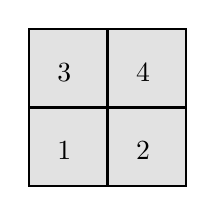
\begin{tikzpicture}
\draw[fill=gray!23,gray!23](0,0) rectangle (2,2);
\draw[thick] (0,0)--(2,0)--(2,2)--(0,2)--cycle;  
\draw[thick] (0,1)--(2,1);  
\draw[thick] (1,0)--(1,2);  
\node[] at (0.45,0.45) {1};
\node[] at (1.45,0.45) {2};
\node[] at (0.45,1.45) {3};
\node[] at (1.45,1.45) {4};
\end{tikzpicture}


\end{center}

The corresponding matrix (making abstraction of the $\beta$ term) writes:
\[
h^2
\left(
\begin{array}{cccc}
2 & -1 & -1 &0 \\
-1 & 2 & 0 & -1 \\
-1 & 0 & 2 & -1 \\
0 & -1 & -1 & 2
\end{array}
\right)
\left(
\begin{array}{c}
p_1 \\ p_2 \\ p_3 \\ p_4
\end{array}
\right)
\]
and the row/column sum of its entries is always nul.
%gresho & sani
This is crucially important to the success of the method since it implies
that the local incompressibility of the $Q_1P_0$ method is retained
after stabilisation (albeit over macro-elements).
It also suggests that a good strategy when constructing the partition 
is to form macro-elements containing as few elements as possible. 
Once a suitable macro-element partitioning has been formed, the local stabilisation
matrices can be calculated by running through the component elements, 
summing jump contributions corresponding to the internal edges. 

If one now considers the following irregular macro-element,
\begin{center}
\begin{flushright} {\tiny {\color{gray} (tikz\_macro2.tex)}} \end{flushright}
%~~~~~~~~~~~~~~~~~~~~~~~~~~~~~~~~~~~~~~~~~~~~~~~~~~~~~~~~~~~~~~~~~~~~~~~~~~~~~~~~~~~~~~~~~~~~~~~~~~


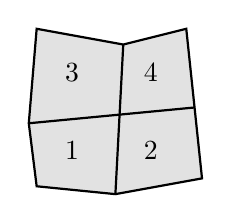
\begin{tikzpicture}
\draw[thick,fill=gray!23] (0,0)--(1,-0.1)--(2.1,0.1)--(1.9,2)--(1.1,1.8)--(0,2)--(-0.1,0.8)--cycle;  
\draw[thick] (-0.1,0.8)--(2,1);  
\draw[thick] (1,-0.1)--(1.1,1.8);  
\node[] at (0.45,0.45) {1};
\node[] at (1.45,0.45) {2};
\node[] at (0.45,1.45) {3};
\node[] at (1.45,1.45) {4};
\end{tikzpicture}




\end{center}


the corresponding matrix is given by\footnote{I suspect it should involve the normal vectors
to the edges ...?}
\[
\tilde{h}
\left(
\begin{array}{cccc}
h_{12}+h_{13} & -h_{12} & -h_{13} & 0\\
-h_{12} & h_{12}+h_{24} & 0 & -h_{24} \\
-h_{13} & 0 & h_{13}+h_{34} & -h_{34} \\
0 & -h_{24} & -h_{34} & h_{24} + h_{34}
\end{array}
\right)
\left(
\begin{array}{c}
p_1 \\ p_2 \\ p_3 \\ p_4
\end{array}
\right)
\]
where $h_{ij}$ is the length/surface of the edge betweens elements $i$ and $j$. 
The reference length $\tilde{h}$ may be computed by simply defining it to be the average 
diameter of the constituent elements. 

%grsa
In three dimensions, the 2x2x2 block is the obvious starting point for stabilising $Q_1P_0$.

Perhaps the most serious potential drawback of the local framework is that 
stability is only guaranteed if the stabilisation parameter $\beta$ is bigger than some 
critical value $\beta_0$, which needs to be estimated.

It can be estimated that $\beta=1/4$ in 2D and $\beta=1/6$ in 3D (see \cite[p636]{grsa} 
for a detailed derivation, see also \cite{vibo92}). 

%sike90
The advantages of the stabilisation procedures over the penalty method 
are especially relevant to the discretisation of 3D incompressible flow problems, 
since iterative solution methods have to be used. 
Similar stabilisation techniques to those described here are applicable to  
the three-dimensional version of the $Q_1P_0$ mixed method.

The conclusion in \cite{sike90} is as follows:
The local jump formulation proves to be an efficient method for a priori filtering of  
spurious pressure modes. It cleanly stabilises the $Q_1\times P_0$ mixed method without compromising 
its simplicity and resulting efficiency; in particular, it is very robust with respect to the magnitude
of the stabilisation parameter. 

It is reported in \cite{grsa} that when using an iterative solver, iteration counts 
are only independent of the grid in the stabilised cases: using the raw $Q_1\times P_0$ method
the iteration counts significantly increase with decreasing $h$. Note that the deterioration
of the condition number of the matrix with decreasing $h$ is worse in 3D than in 2D (but
bear in mind that one almost always use higher resolutions in 2D than in 3D, so it does not help).




A way to look at the global vs. local stabilisation schemes is presented 
on the following figure from Christon (2002) \cite{chri02}:

\begin{center}
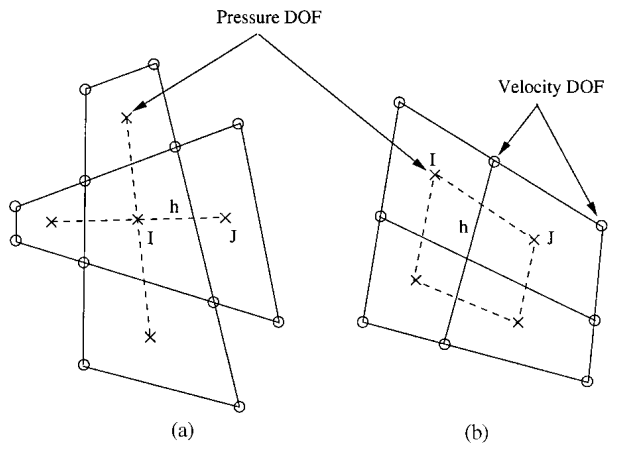
\includegraphics[width=10cm]{images/q1p0stab/chri02}\\
{\captionfont Element configuration for pressure stabilization: (a) global jump; (b) local jump.}
\end{center}

\begin{center}
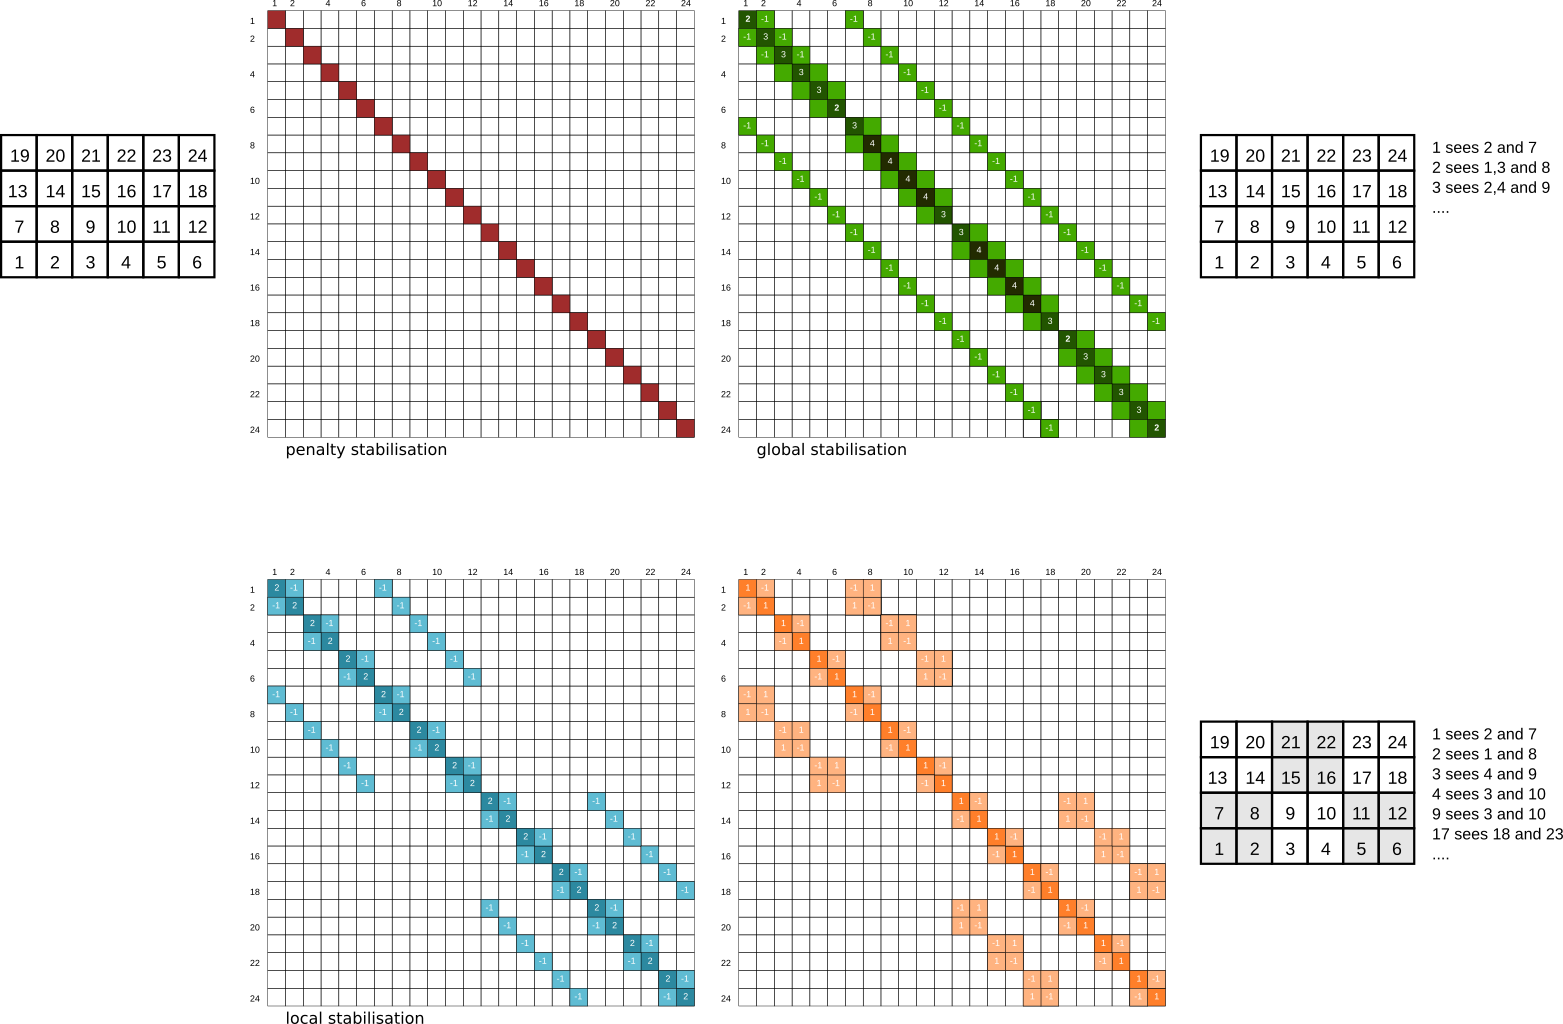
\includegraphics[width=15cm]{images/q1p0stab/stabs.png}
\end{center}


%.................................................
\paragraph{Scaling of the stabilisation matrix}

Looking at the following saddle point problem,
\[
\left( \begin{array}{cc}
\K & \G  \\ 
\G^T & -\C
\end{array} \right) \cdot
\left( \begin{array}{c}  \vec{\cal V} \\ \vec{\cal P}  \end{array} \right) = 
\left( \begin{array}{c}  \vec{f} \\ \vec{g} \end{array} \right) 
\]
where $\C$ is the stabilisation matrix,
the pressure Schur complement equation writes:

\fbox{
\parbox{6cm}{
\[
(\G^T \cdot \K^{-1} \cdot \G  + \C ) \cdot  \vec{\cal P} 
= \K^{-1}\cdot \G \cdot \vec{f} - \vec{h}
\]
}}

Dimensionless analysis: $\K \sim \eta$, $\G_{el} \sim h$, $\C \sim h^{dim}/\eta$, everything is fine.

Since the matrix $\mathbb{K}$ contains the viscosity, it is to be expected that 
the matrix $\mathbb{C}$ somehow follows the values in the $\mathbb{G}^T \mathbb{K}^{-1} \mathbb{G}$  term.
This is indeed what is advocated in Christon (2002) \cite{chri02}:
\[
\C_{ij} = \beta (\G^T\cdot \K^{-1} \cdot \G)_{ij} 
\frac{1}{\Gamma_{ij}} \int_{\Gamma_{ij}} [[\psi_i]]\;[[\psi_j]] d\Gamma
\]
where $i$ and $j$ identify adjacent elements that share a common face.
Here, $\Gamma_{ij}$ represents the shared inter-element boundary, $[[.]]$ is the jump operator,
and $\beta$ is a non-dimensional scaling parameter.
For the $Q_1\times P_0$ element, the pressure approximation is piecewise constant
with $\psi_i=1$ inside the element and zero outside.

The inclusion of the $\G^T\times \K^{-1} \cdot \G$
term (also named pressure-Poisson equation, or PPE) in the stabilisation yields proper 
dimensionality of the stabilization matrix,
accounts for scaling due to irregular elements, and still preserves the symmetry \cite{chri02}.

Note that if one wishes to compute $\C=\mathbb{G}^T \mathbb{K}^{-1} \mathbb{G}$
at the elemental level for $Q_1\times P_0$ elements, it simply boils down to a scalar,
which is rather convenient as it gives in a simple way the scaling for the
stabilisation term.

Per element, $\G_{el}=\frac{h}{2}(+1,+1-1,+1,-1,-1,+1,-1)$, which is also 
presented as Eq (4.3) in Cao (2003) \cite{cao03}, albeit in a different form.
Similarly one obtains (taking $\eta=1$):
\[
\K_{el}
=
\frac{1}{4}
\left(
\begin{array}{cccccccc}
4   & 1   & -2 & -1 & -2& -1 &0  & 1\\
1   & 4   & 1  & 0  & -1& -2 &-1 & -2\\
-2  & 1   & 4  & -1 & 0 & -1 &-2 & 1\\
-1  & 0   & -1 & 4  & 1 & -2 &1  & -2\\
-2  & -1  & 0  & 1  & 4 & 1  &-2 & -1\\
-1  & -2  & -1 & -2 & 1 & 4  &1  & 0\\
0   & -1  & -2 & 1  & -2& 1  &4  & -1\\
1   & -2  & 1  & -2 & -1& 0  &-1 & 4 \\
\end{array}
\right)
\]
Taking $\mathbb{K}_{el}^{-1}=1/diag(\mathbb{K}_{el})$, 
it is easy to (numerically) verify that (at least for square Q1P0 elements) 
the PPE simple writes $\tilde{C} = 2 h^2/\eta $.

It can be proven that the ideal value for the stabilisation parameter is given by $\beta=1/4$ \cite[p241]{elsw}.

Similar approach is taken in \cite{chsu97}

%..............................................
\paragraph{Consistency and stabilisation}


To ensure consistency it is required that  ${\bm 1}\in null(\C)$
and this precludes the use of the penalty method \cite[p239]{elsw}.

Indeed, looking at the 'red' matrix, one sees that $\mathbb{C}\cdot {\bm 1} \neq 0$
where ${\bm 1}=(1,1,1,...1)$.
Interestingly the green and blue matrices corresponding to the global and local
stabilisation schemes do verify $\mathbb{C}\cdot {\bm 1} = 0$ (the sum
of each row is strictly zero).

To provide stabilisation, it is required that
$\vec{\cal P}_\star \cdot \C \cdot \vec{\cal P}_\star > 0$ for all
spurious pressure modes $\vec{\cal P}_\star \neq 1$ in $null(\G)$ \cite[p239]{elsw}.


%..............................................
\paragraph{In three dimensions}


The matrix $\SSS$ is obtained by assembling the submatrices 
for the macroelements which, in general, are made up of 8 (i.e., 2x2x2) 
adjacent elements, as shown in the following sketch \cite{chsu97}:

\begin{center}
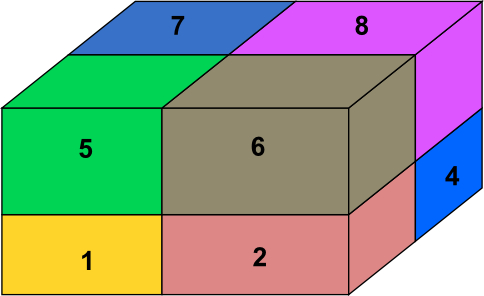
\includegraphics[width=4cm]{images/q1p0stab/macro3D}\\
{\captionfont Numbering of hexahedrons in a macroelement.\\ 
Element No. 3 is behind No. 1 and below No. 7.} 
\end{center}

For a macroelement of 8 elements as ordered in the above sketch, the submatrix is defined below:

\[
\SSS=
\left(
\begin{array}{cccccccc}
h_{12}+h_{13}+h_{h15} & -h_{12} & -h_{13} &  0  &  -h_{15} & 0  & 0 & 0 \\
-h_{21} & h_{21}+h_{24} + h_{26} & 0 & -h_{24} & 0 & -h_{26} & 0 & 0 \\
-h_{31} & ... \\
0 & ... \\
-h_{51} & ...\\
0 & ...\\
0 & ...\\
0 & ...
\end{array}
\right)
\]
in which $h_{ij}$ is the length scale for elements ‘i’ and ‘j’ in the macroelement. 
The matrix $\SSS$ is symmetric, since $h_{ij}=h_{ji}$. 

Two approaches are possible  for computing the length scale $h_{ij}$:
\begin{itemize}
\item the square root of the interior inter-element surface area between elements ‘i’ and ‘j’
\item the quotient of the interior inter-element surface area divided by the cube 
root of the average element volume of the macroelement.
\end{itemize}


%.............................................................................
\paragraph{The stabilisation matrix in the presence of viscosity contrasts}

The previously advocated scaling of the $\C$ matrix is not clear when it comes to viscosity contrasts
from one element to the other. When using a Conjugate Gradient method for the outer iterations, 
the matrix $\C$ must be SPD. However, scaling the row entries of the $\C$ matrix by the element 
viscosity still yields a structurally symmetric matrix, but not a numerically symmetric one !
Some form of viscosity averaging must then take place between adjacent elements so that the contribution 
from elt A to B in exactly the same as B to A.  

However, in order for the stabilisation to remain consistent (FIND SOURCE) it must 
satisfy $\C\cdot \vec{1}= 0$, 
i.e. it should have zero effect on a constant pressure field, which simply forces
the sum of the entries for each row to be nul. This requirement makes the above viscosity averaging 
idea very difficult in practice in the global case (satisfying both symmetry and consistency).

In the global stabilisation case, a reference viscosity valid for the whole domain should be used. 

In the local stabilisation approach, each macro-element is 'isolated' from the others so that an average
viscosity can be computed for each block of 4 (2D) or 8 (3D) elements and used to scale the $\C$ matrix
yielding a symmetric matrix and a consistent one too.
Let us look at the following patch of elements. Each macro-element is assigned an average viscosity
(represented by a different colour for each), 
function of the elemental viscosities within the macro-element. 

\begin{center}
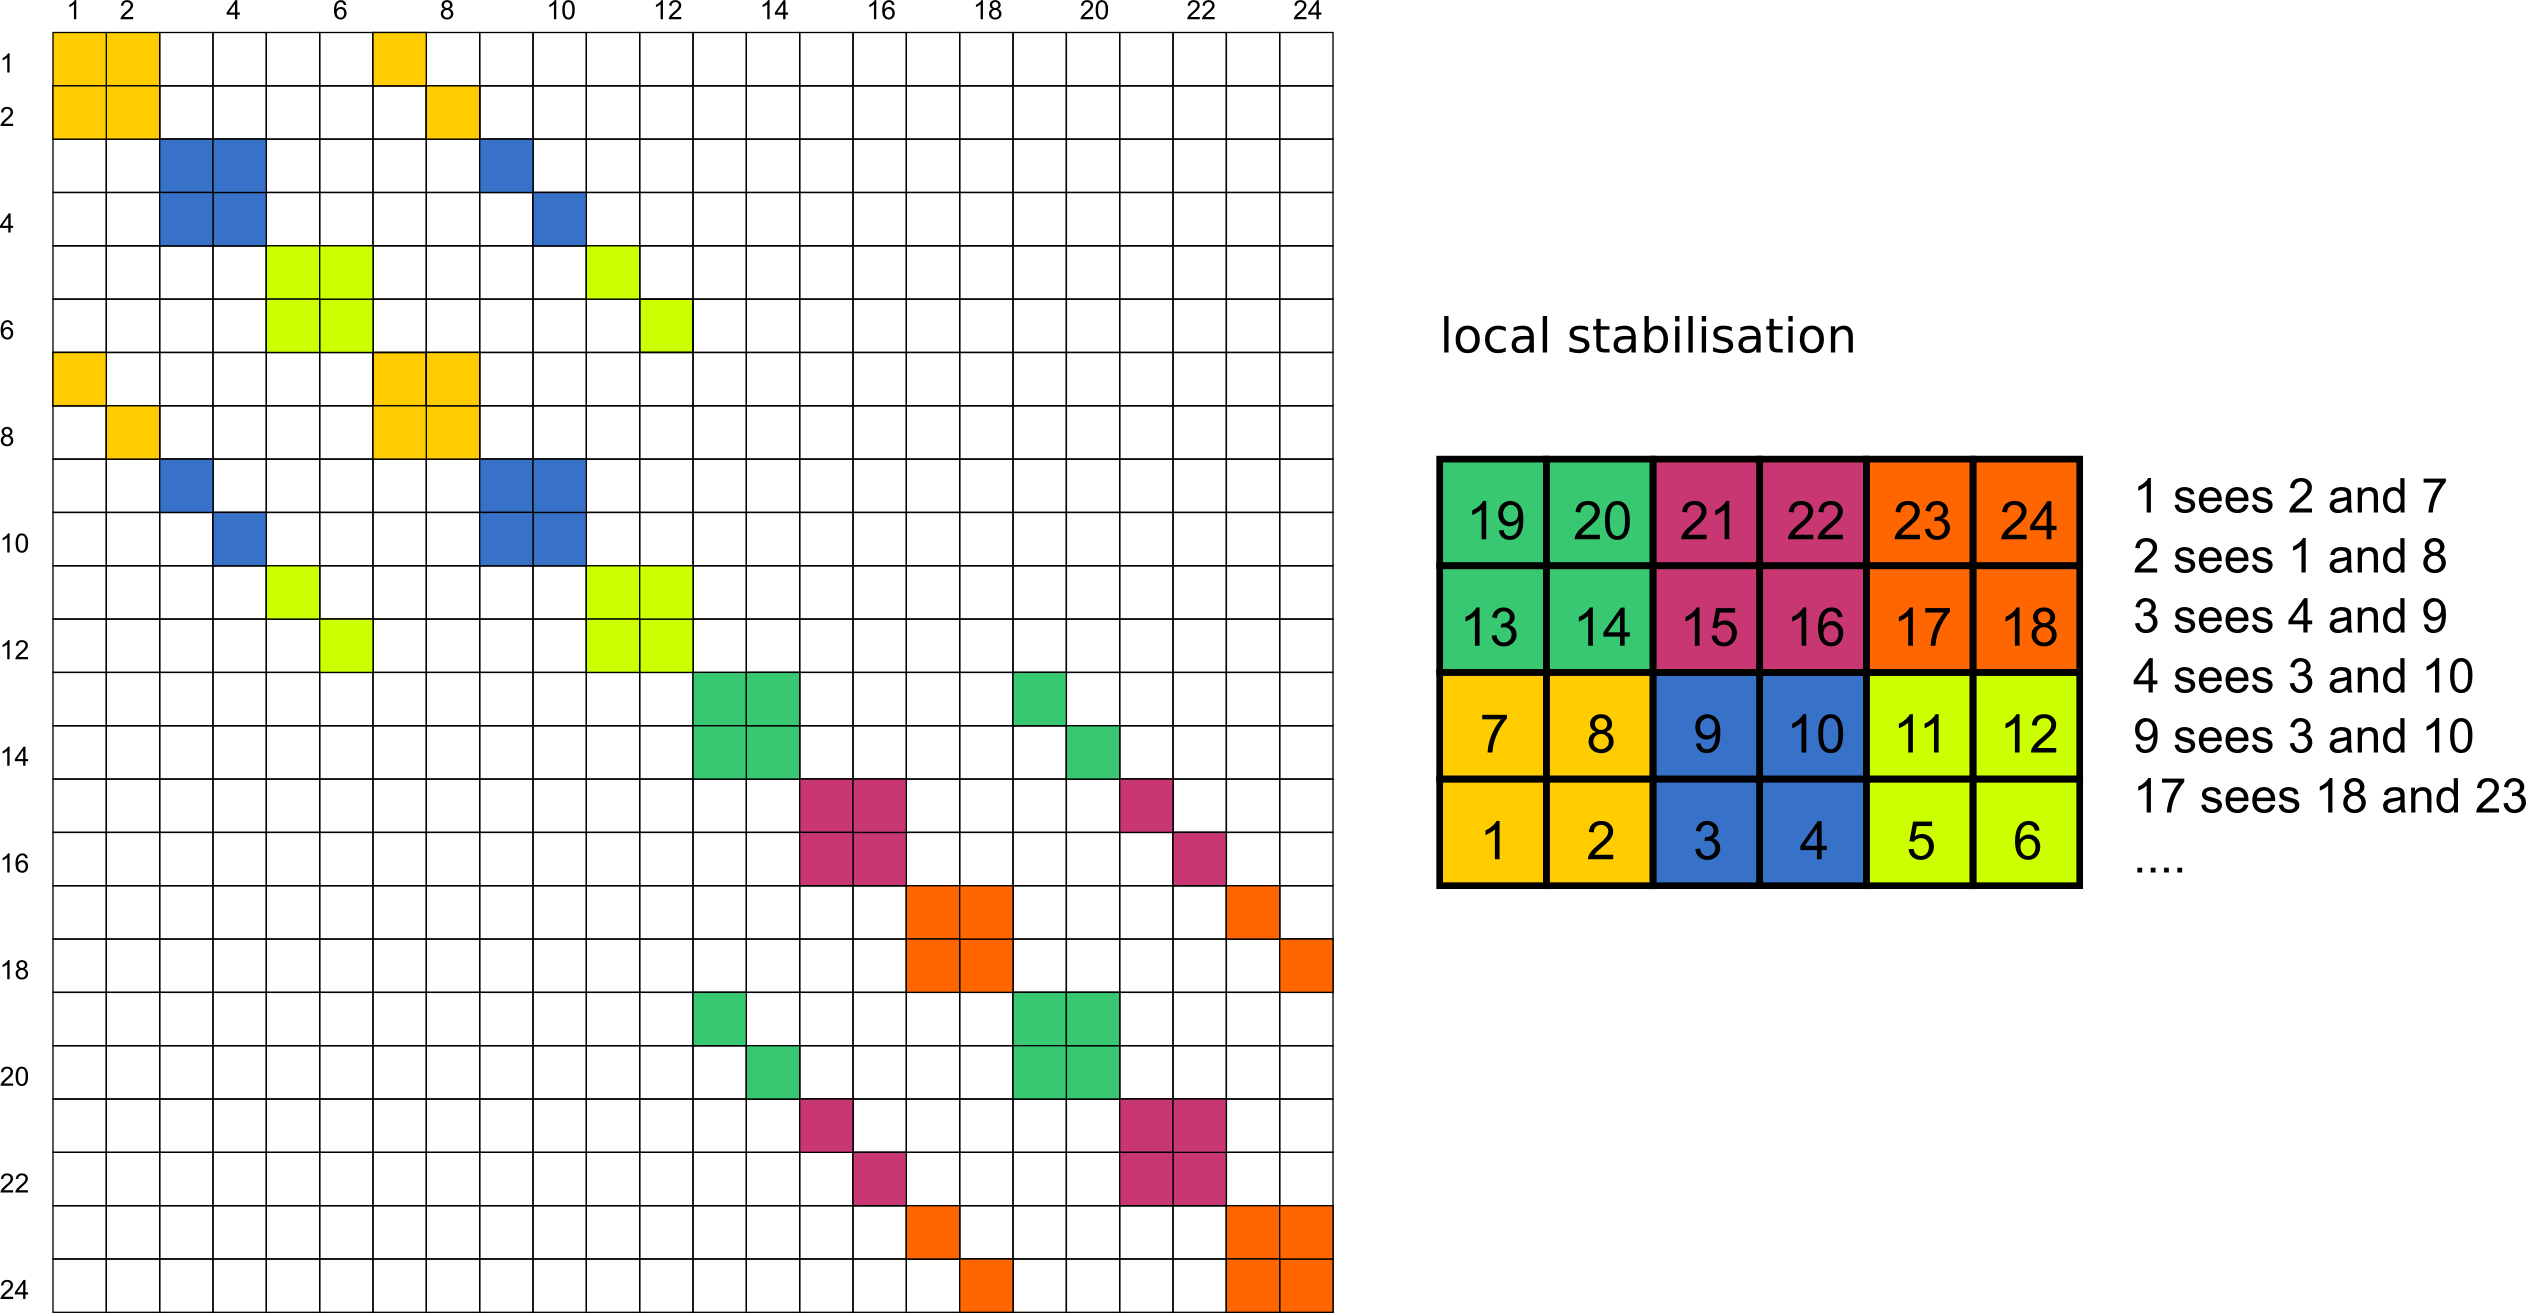
\includegraphics[width=15cm]{images/q1p0stab/stab_local.png}
\end{center}

In the matrix $\C$ the nonzero values are also shown with the corresponding colours.
The matrix symmetry is preserved: elt 1 sees 2 and vice versa, but the prefactor is the same, corresponding
to the yellow colour. Each row of the matrix contains only one colour, thereby preserving consistency.
 
REMARK: I suspect the matrix is still SPD as it is the previous matrix multiplied by a diagonal matrix.



This approach is now abandonned. The solution (or at least) the inspiration came from Christon (2002) \cite{chri02}.The author gives his recipe to scale the $\C$ matrix:

\begin{center}
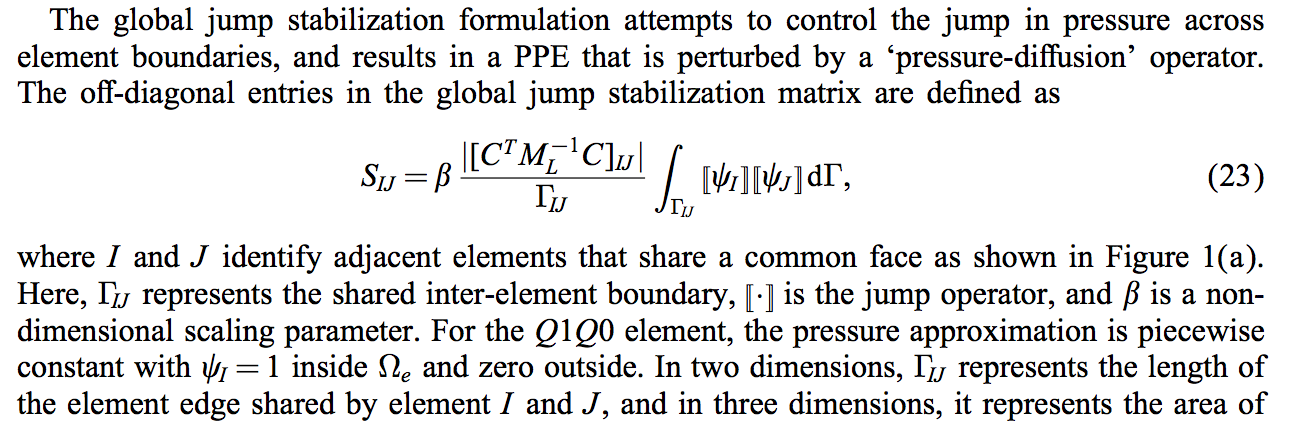
\includegraphics[width=15cm]{images/q1p0stab/chri_a.png}\\
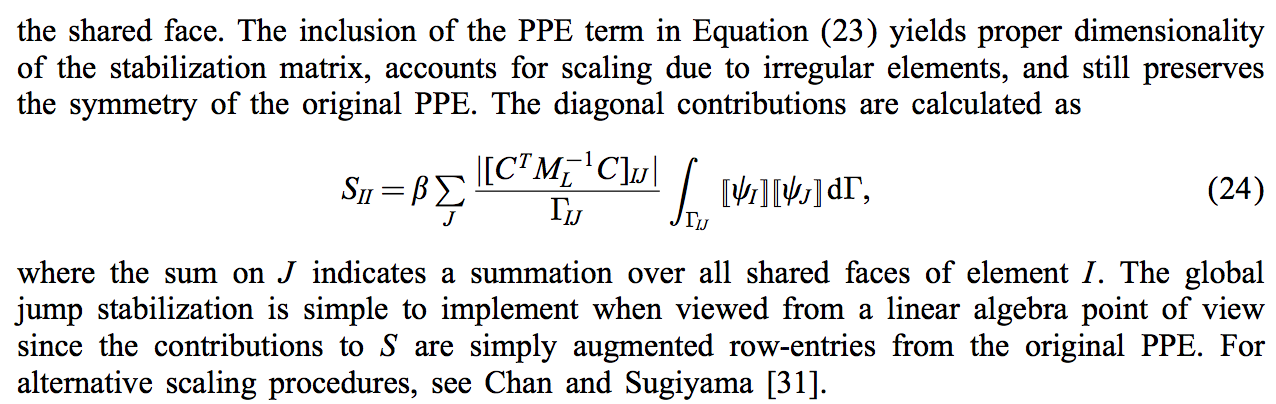
\includegraphics[width=15cm]{images/q1p0stab/chri_b.png}
\end{center}

I however find this method unpractical because one needs to compute the
Schur complement $\G^T \K^{-1} \G$ (or $C^T M_L^{-1} C$ in his case).
I suspect he does not really build it but he remains evasive on his 
workaround. 
I need to find an approximate expression. I first replace $\K$ by
its diagonal $\K_d$: $\G^T \K_d^{-1} \G$. The diagonal contains 
positive terms proportional to the dynamic viscosity. Its inverse 
is simply a diagonal matrix containing the inverse of the terms.
One can therefore write: 
\begin{eqnarray}
\G^T \K_d^{-1} \G 
&=& \G^T \sqrt{\K_d}^{-1} \sqrt{\K_d}^{-1} \G  \nn\\
&=& ( \sqrt{\K_d}^{-1} \G)^T (\sqrt{\K_d}^{-1} \G)  \nn\\
\end{eqnarray}

We know that $\G \sim h$ (in amplitude) and that $\K \sim \mu$ so that
$ \G^T \K_d^{-1} \G \sim h^2/\mu$. 
The $(IJ)$ component of this matrix will then be approximated by
$(\G^T \K_d^{-1} \G)_{IJ} \sim  h^2/\sqrt{\mu_I \mu_J} $. 
This has the added benefit that it yields a symmetric matrix too
(the $IJ$ component is equal to the $JI$ component).
However, there is no guarantee of consistency (i.e. the sum of the
terms on a row do not necessarily add up to zero). 
Diagonal terms are therefore computed as in Eq. (24) of \cite{chri02}.


